\chapter[Analiza zmogljivosti obla"cne storitve c9]{Analiza zmogljivosti obla"cne storitve Cloud9}

\pagestyle{fancy}
\fancyhf{}
\fancyhead[LE,RO]{\thepage}
\fancyhead[RE,LO]{\leftmark}

\huge "Ziga Kokelj, Tadej Hiti,\\Miha Bizjak, Matej Kristan
\normalsize
\bigskip

\section{Opis problema} \label{8_opis_problema}
\noindent Dana"snje dni se vse bolj uveljavljajo obla"cne storitve, saj so s stali"s"ca uporabnika najenostavnej"se za uporabo. Na"sa naloga je implementirati prenos datoteke na oz. z obla"cne storitve in breme na obla"cni storitvi, za katero smo si izbrali sortiranje numeri"cnih podatkov.
\noindent Na sliki \ref{8_opis_problema} je grafi"cen prikaz opisanega problema.
\noindent Na"se testiranje bo obsegalo merjenje razli"cnih izvajalnih "casov na podlagi katerih bi pri"sli do podatkov o zmogljivosti sistema. Breme obla"cnega sistema bodo datoteke razli"cnih velikosti, ki bodo vsebovale naklju"cno generirana "stevila. Obla"cna storitev pa bo vsebine datotek uredila po izbranem algoritmu za urejanje "stevil.  
Namen na"se naloge je ugotoviti zmogljivost zastonjske obla"cne storitve z vidika razli"cnih metrik. 

\begin{figure}
  \centering
    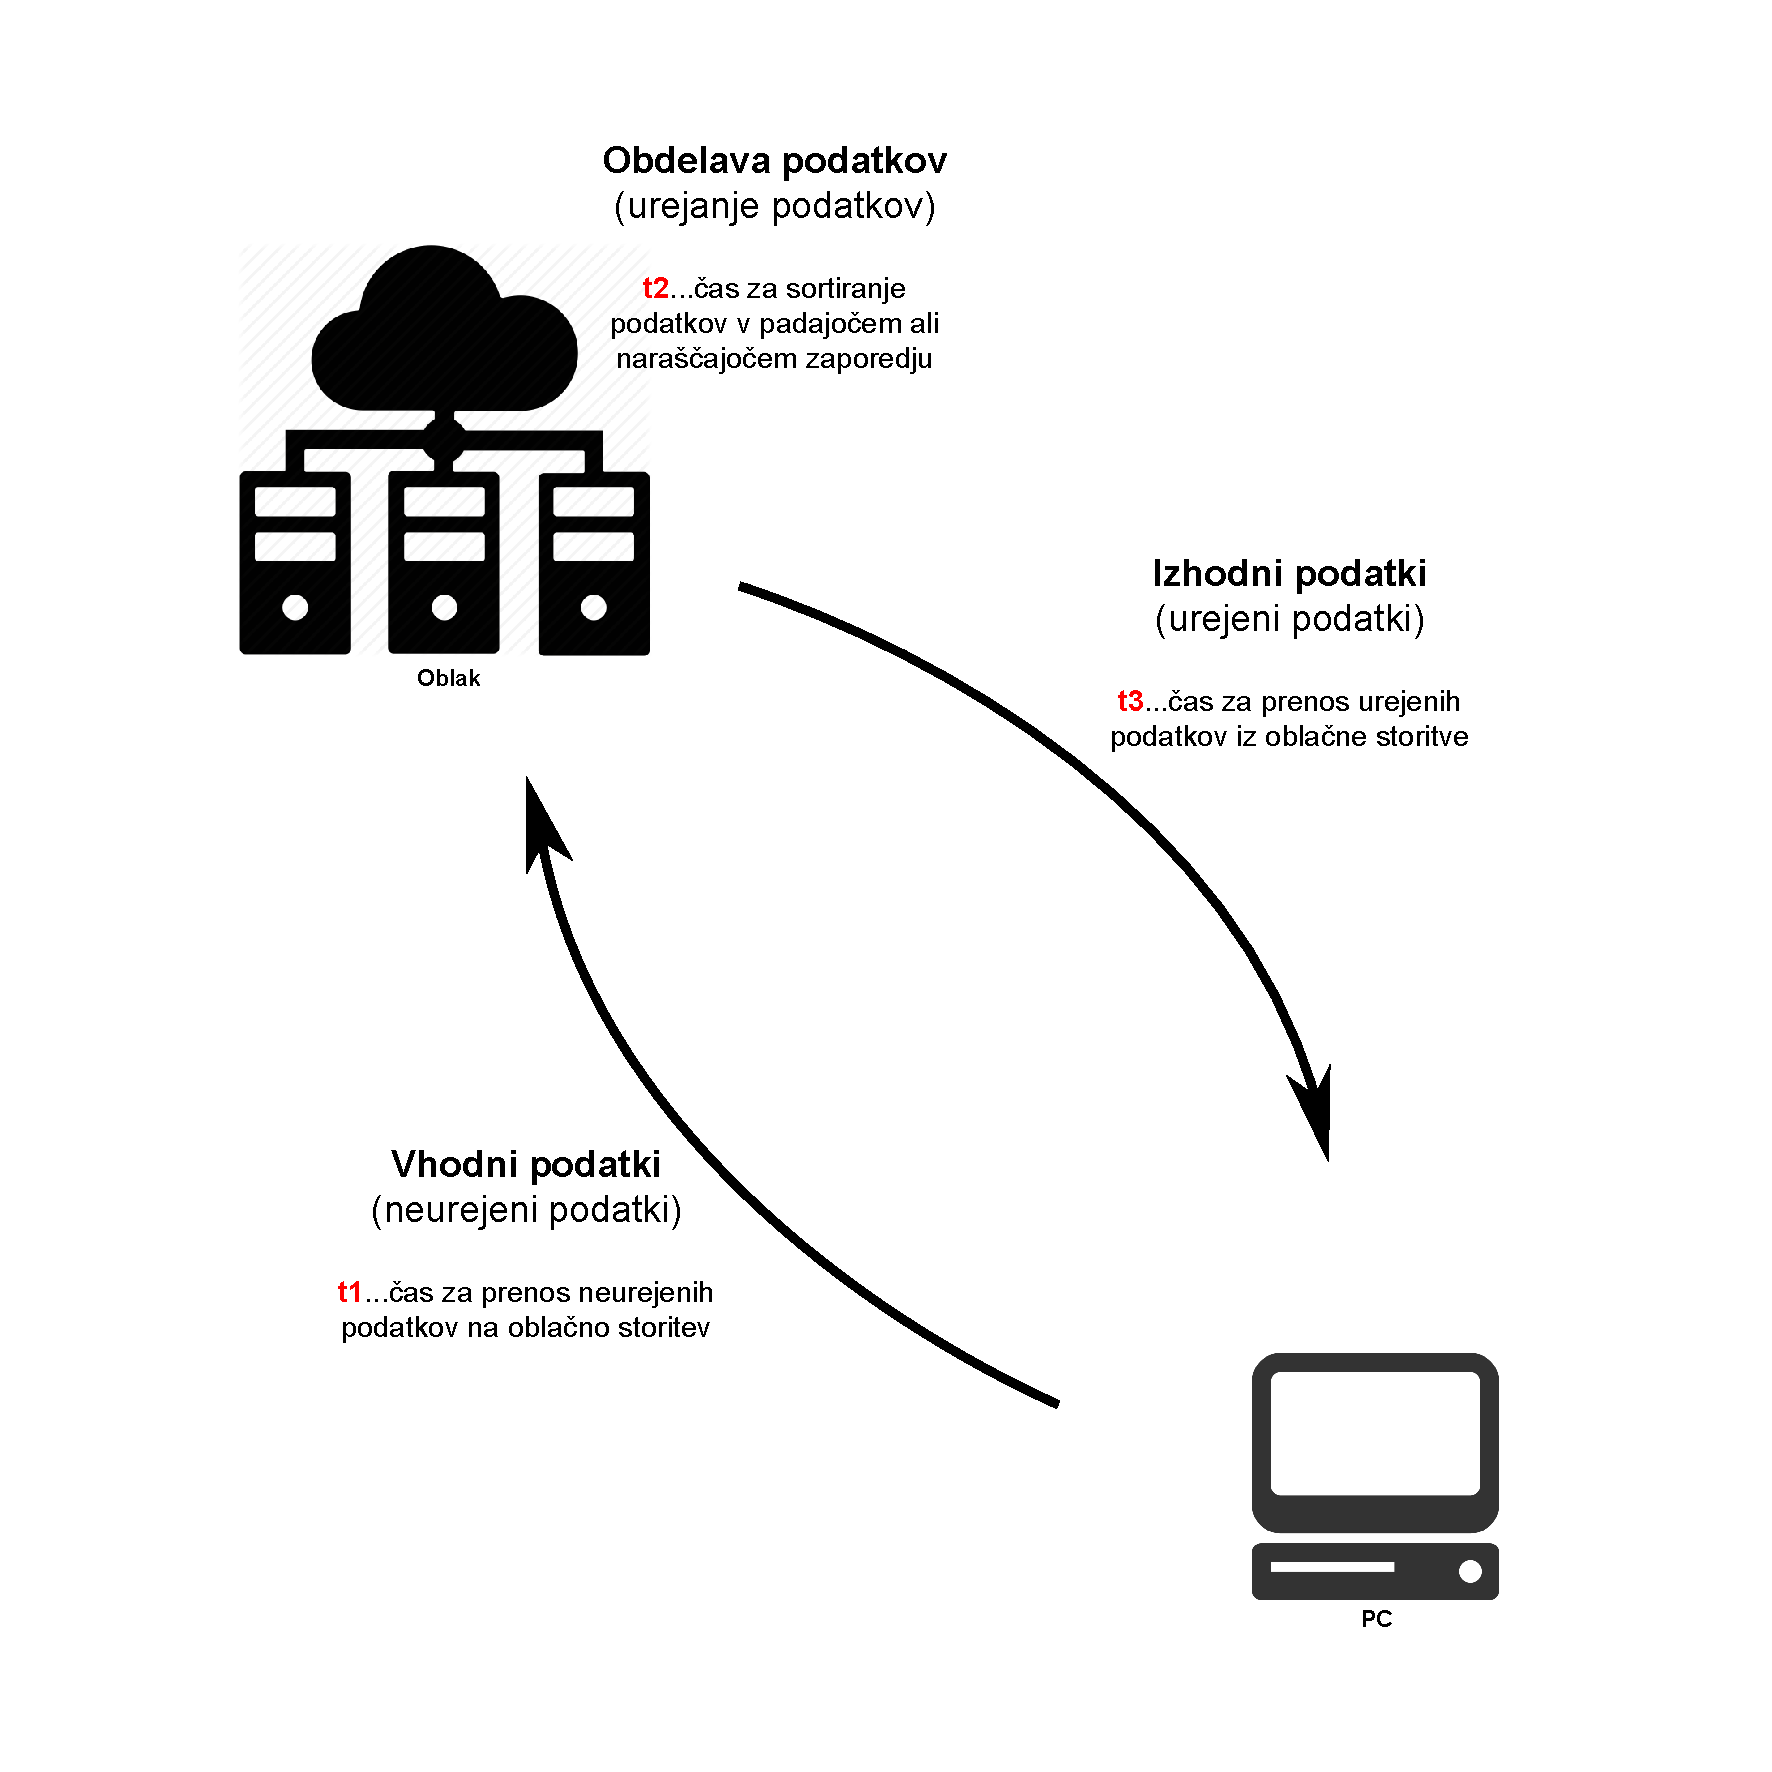
\includegraphics[width=0.74\textwidth]{8_zzrs_opis_problema.pdf}
  \caption{Shema delovanja sistema.}
  \label{8_opis_problema}
\end{figure}


\section{Izbira ponudnikov}
Zaradi predhodnih izku"senj z obla"cno storitvijo Cloud9 smo se odlo"cili za njihovo zastonjsko ponudbo. Cloud9 ponuja razvojno okolje in operacijski sistem Ubuntu v katerem lahko pi"semo ali pa izvajamo razli"cne programe.  Pri brezpla"cni naro"cnini nam dajo v uporabo 512MB RAM-a in 2GB prostora na disku.


\section{Izbira tehnologij}
V tem razdelku so na kratko opisane vse izbrane tehnologije, ki smo jih realizirali za na"so analizo.

\subsection{Tehnologija v oblaku}
V obla"cni storitvi smo implementirali stre"znik, ki je napisan v jeziku javascript z uporabo knji"znice Node.js~\cite{8_nodejs}. Stre"znik od uporabnika sprejme datoteko, jo avtomatsko sortira z dolo"cenim algoritmom za sortiranje "stevil ter nato sortirano datoteko po"slje nazaj uporabniku. 

\subsection{Tehnologija za avtomatizacijo odjemalcev}
Zaradi avtomatskega testiranja smo napisali skripto v programskem jeziku python~\cite{8_python}, ki omogo"ca avtomatsko po"siljanje datoteke in URL zahteve na stre"znik, ter kot odgovor prejme urejeno datoteko z urejenimi podatki. Seveda ob tem zabele"zimo "se "cas pred po"siljanjem zahteve in "cas po prejetju urejene datoteke, da dobimo izvajalni "cas celotne procedure. Ker je odjemalcev lahko ve"cje "stevilo, smo ta problem re"sili z nitmi, kjer vsaka nit predstavlja enega odjemalca in po"silja zahteve na stre"znik.

\section{Rezultati meritev}
V tem razdelku so opisani na"cin testiranja na"se  storitve in rezultati meritev.

\subsection{Testiranje I.}
Naklju"cno smo generirali po eno datoteko z 10000/15000/20000/25000/30000 integer "stevili, ki jih je nato 10/20/30/40/50 odjemalcev po"siljalo na stre"znik. Izmerili smo "case potrebne za prejetje urejene datoteke in pri"sli do povre"cnih "casov. Testiranje je bilo izvedeno ob8 ih zjutraj V Ljubljani v sredo 3.5.2017. Vse meritve so prikazane na sliki \ref{8_test1} in v tabelah \ref{8_table1}, \ref{8_table2}, kjer je prikazan povpre"cen "cas obdelave. Pri vseh testiranjih se je uporabilo 10 razli"cnih vnaprej naklju"cno generiranih datotek. Za sortiranje "stevil se uporablja algoritem bubble sort. 
 Pri datotekah z ve"c stevili in veliko odjemalci je prihajalo do nekaterih napak, ki jih trenutno "se odpravljamo.\\\\

\begin{figure}
  \centering
    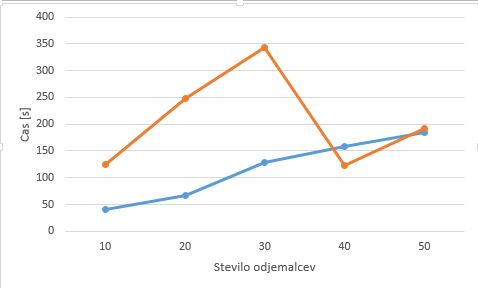
\includegraphics[width=0.65\textwidth]{testiranje_int.jpg}
  \caption{Graf "casa obdelave v odvisnosti od "stevila odjemalcev.}
  \label{8_test1}  
\end{figure}

\begin{figure}[!htbp]
  \centering
  \begin{tabular}{ | c | c | c | }
    \hline
    "Stevilo odjemalcev & Povpre"cni cas obdelave[s] & Standardna deviacija\\ \hline
    10 & 41.3034 & 1.0168 \\ \hline
    20 & 66.1481 & 1.7781 \\ \hline
    30 & 127.7942 & 8.3947 \\ \hline
    40 &158.8352 &  6.2111\\ \hline
    50 & 184.7879 &  3.6371\\ \hline
  \end{tabular}
  \caption{Tabela "casov obdelav datoteke z 10 tiso"c integer "stevili.}
  \label{8_table1}
  \centering
\end{figure}

\begin{figure}[!htbp]
  \centering
  \begin{tabular}{ | c | c | c | }
    \hline
    "Stevilo odjemalcev & Povpre"cni cas obdelave[s] & Standardna deviacija\\ \hline
    10 & 124.4322 & 2.7692 \\ \hline
    20 & 248.6854 & 10.797 \\ \hline
    30 & 344.0970 & 19.4963 \\ \hline
    40 & 123.3930 & 21.8550\\ \hline
    50 & 192.7521 & 23.4215\\ \hline
  \end{tabular}
  \caption{Tabela "casov obdelav datoteke z 20 tiso"c integer "stevili.}
  \label{8_table2}
  \centering
\end{figure}

\section{Plan za prihodnje delo}
V prihodnje moramo odkriti in odpraviti te"zave pri testiranju ve"cjih datotek z veliko odjemalci. Po odpravljenih te"zavah pa bo potrebno izvesti "se ve"c testov v razli"cnih delih dneva in iz razli"cnih lokacij po Sloveniji, da bomo podatke lahko primerjali med seboj. \\
